\chapter{Methods}
\label{chapter:methods}
In the following, we present a model for the transmission of methylation patterns by \acfp{DNMT}, depending on four parameter, which characterize the function of these \acp{DNMT}. Based on that, two computational methods are provided to identify the most realistic way to choose the parameters compared to some real-world methylation data. The aim of this paper is not only to compute the model parameters, but also to compare different approaches to retrieve and evaluate them.

\section{Model}
\label{Model}
The model underlies the following procedure:
\begin{enumerate}
\item initially a double-stranded, partially methylated DNA sequence with multiple \acfp{CpG} is given
\item one of the strands serves as template for the methylation of a second yet unmethylated strand
\item the three \acp{DNMT} DNMT1, DNMT3a and DNMT3b eventually bind and methylate along the DNA strand
\item the cell divides and step three starts again
\end{enumerate}
Basically, each \acf{bp} is one state of the model, in which the binding state of the \acp{DNMT}is kept and if this position is part of a \ac{CpG}. If the second condition holds, the current methylation state is stored. It is assumed, there are four possible methylation states for one \ac{CpG}/\ac{CpG}-dyad. Either none of the cytosines are methylated, then the dyad is unmethylated or the cytosine at the parental or daughter strand is methylated and the respectively other one not, then the \ac{CpG} is called hemimethylated. In the final case, both cytosines are methylated, which corresponds to a fully methylated dyad. The methylation states are encoded in the following way:\newline
\begin{align}
m_i := \text{methylation state of dyad i}\\
m_i = \left\{
\begin{array}{l}
\text{0 unmethylated} \\
\text{1 hemimethylated, methylation on parent strand} \\
\text{2 hemimethylated, methylation on daughter strand} \\
\text{3 fully methylated}
\end{array}
\right.
\end{align}

\begin{figure}[h]
\centering
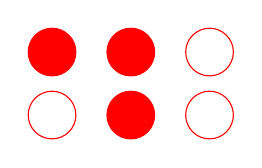
\begin{tikzpicture}
  \draw[red, fill=red](-1,0)circle(2ex);
  \draw[red](-1,-0.8)circle(2ex);
  \draw[red, fill=red](0,0)circle(2ex);
  \draw[red, fill=red](0,-0.8)circle(2ex);
  \draw[red](1,0)circle(2ex);
  \draw[red](1,-0.8)circle(2ex);
\end{tikzpicture}
\caption{A methylation pattern with three CpGs; each circle represents one CpG; plane red circles are methylated CpGs; the pattern code is 28 and is computed as $1*4^2 + 3*4^1 + 0*4^0 = 16 + 12 + 0 = 28$}
\label{fig:mexample}
\end{figure}

The different methylation patterns in figure \ref{fig:methylationpatterns}, whereby subfigure \ref{fig:sfig0} corresponds to pattern 0 and so on.\newline
In this way, the full methylation pattern M of a DNA sequence can be encoded as a number in range $4^(L-1)$, where L is the number of \acp{CpG}. The code can be interpreted as sum over the methylation states. Hereby the rightmost dyad is the zeroth dyad and all following methylation states are shifted by 2 bits times the enumeration of the dyad (see an example in figure \ref{fig:mexample}).
\[M = \sum^{L-1}_{i=0}{m_i * 4^{L-1-i}}\]
\begin{figure}
X = \{0:0.2, 1:0.01, 3:0.02, 11:0.1, 14:0.05, 35:0.01, 36:0.21, 56:0.15, 57:0.05, 63:0.2\}
\label{dict}
\caption{methylation pattern distribution X of a locus with 3 CpGs; each key represents one methylation pattern, the following number the frequency of this pattern; the patterns not listed have frequency zero; assuming, there are 100 samples, the patterns have a absolute frequency of 20, 1, 2, 1, 5, 1, 21, 15, 5 and 2 respectively.}
\end{figure}
If we are given a set of methylation patterns, the pattern distribution may be represented as dictionary, where the key of each entry is a methylation pattern and its value the frequency of this key in the set of methylation patterns. See Figure \ref{dict} for an example.\\

Further, it is assumed two methyltransferases are active, DNMT1 and DNMT3. For simplification, no other enzymes are included in the model, thus there may be enzymes which influence the methylation process. In earlier experiments it was shown that DNMT1 binds to the daughter strand, whereas DNMT3 is able to bind to both strands (see section \ref{section:DNAMeth}). This knowledge is included by recognizing the binding state of each enzyme to their strands.\newline
Therefore, each state of a \ac{CpG} can be stored as a combination of four numbers, where the numbers contribute to the methylation state, the binding state of DNMT1 to the new strand and DNMT3 to the old and new strand respectively.
\begin{align*}
S_i := \text{state of dyad i}\\
S_i = (m_i, B1_i, B3p_i, B3d_i)\\
m \in \{0,1,2,3\}^L\\
B1 \in \{0,1\}^L\\
B3p \in \{0,1\}^L\\
B3d \in \{0,1\}^L
\end{align*}
Here B1 is the binding state of DNMT1 and B3p the binding state of DNMT3 to the parental strand and B3d the binding state to of DNMT3 to the daughter strand. Zero and one signify an unbound and bound enzyme.\\

%de novo/maintenance
\begin{figure}[h]
\centering
\begin{tikzpicture}[>=stealth',bend angle=45,auto,->,shorten >=1pt]
  \tikzstyle{place}=[circle,thick,draw=black!75,minimum size=6mm,font=\large]
  \node [place](0)at (0,0){0};
  \node [place](1)at (1.5,0.8){1};
  \node [place](2)at (1.5,-0.8){2};
  \node [place](3)at (3,0){3};
  \path (0)edge node{$\delta$}(1)
  		   edge node{$\delta$}(2)
  		(1)edge node{$\mu$}(3)
  	    (2)edge node{$\mu$}(3);
\end{tikzpicture}
\caption{Possible transitions between the methylation patterns of a dyad; the numbers represent the methylation patterns m; each transition shows a possible methylation with the probability denoted on the arrow}
\label{mhy}
\end{figure}
Two kinds of methylations are distinguished in the model. The methylation of a cytosine is called maintenance if the opposite base is yet methylated. Contrary, if the opposite base is unmethylated, the methylation event is called de novo. And the probabilities of each event are denoted by $\mu$ and $\delta$, consistent to earlier approaches (\ref{section:RelWork}). Figure \ref{mhy} shows the resulting possible transitions.\\

%rho/tau
\begin{figure}[h]
\centering
\begin{tikzpicture}[>=stealth',bend angle=45,auto,shorten >=1pt]
  \tikzstyle{place}=[circle,thick,draw=black!75,minimum size=6mm,align=center]
  \tikzstyle{red}=[circle,thick,draw=red!75,minimum size=6mm,align=center, text=red]
  \draw[thick] (0,0) -- (9,0) node[anchor=north west]{position(bp)};
  \foreach \x in {0,1,2}
   \draw (\x *3+1,1pt) -- (\x *3+1,-1pt) node[anchor=north] {$\x$};
  \node [place](0u)at (1,4){DNMT\\ unbound};
  \node [place](1u)at (4,4){DNMT\\ unbound};
  \node [place](2u)at (7,4){DNMT\\ unbound};
  \node [red](0b)at (1,1){DNMT\\ bound};
  \node [red](1b)at (4,1){DNMT\\ bound};
  \node [red](2b)at (7,1){DNMT\\ bound};
  \path[->] (0b)edge node{$\rho$}(0u)
  		   edge node{$1-\rho$}(1b)
  		(1b)edge node{$\rho$}(1u)
  		   edge node{$1-\rho$}(2b)
  		(2b)edge node{$\rho$}(2u)
  		(0u)edge node{$1-\tau$}(1u)
  			edge node{$\tau$}(1b)
  		(1u)edge node{$1-\tau$}(2u)
  			edge node{$\tau$}(2b);
\end{tikzpicture}
\caption{Transitions between the binding states of a DNMT over the DNA; each number represents one bp on the strand; red circles symbolize that DNMT is bound to the DNA at that position, black ones are unbound enzymes; the arrows show possible transitions between the binding states}
\label{rho}
\end{figure}
The probabilities of attachment and disattachment of a \ac{DNMT} are defined as $\tau$ and $\rho$. Therefore, the association length, the number of \acp{bp} where the enzyme is bound is $1/\rho$ and the probability that the \ac{DNMT} stays bound at one \ac{bp} and its neighbour is 1-$\rho$. This parameter setting is similar to the approach of Fu et al. from 2012.\cite{Fu} Figure \ref{rho} visualises the binding states and their probabilities.\\

%Alle Übergänge 
\begin{figure}[h]
\begin{tabularx}{\textwidth}{l|c|c|c|c}
\multicolumn{5}{c}{\textbf{$m_i$}}\\
\cline{2-5}
\textbf{($m_i, B1_i, B3p_i, B3d_i$)}&	0&	1&	2&	3\\
\hline
(0, 0, 0, 0)&	1&	0&	0&	0\\
(0, 0, 0, 1)&	$1-\delta_d$&	0&	$\delta_d$&	0\\
(0, 0, 1, 0)&	$1-\delta_p$&	$\delta_p$&	0&	0\\
(0, 0, 1, 1)&	$(1-\delta_p)(1-\delta_d)$&	$\delta_p(1-\delta_d)$&	$\delta_d(1-\delta_p)$&	$\delta_p \delta_d$\\
(0, 1, 0, 0)&	1&	0&	0&	0\\
(0, 1, 0, 1)&	$1-\delta_d$&	0&	$\delta_d$&	0\\
(0, 1, 1, 0)&	$(1-\delta_p)$&	$\delta_p$&	0& 0\\
(0, 1, 1, 1)&	$(1-\delta_p)(1-\delta_d)$&	$\delta_p(1-\delta_d)$&	$\delta_p(1-\delta_d)$&	$\delta_p \delta_d$\\
(1, 0, 0, 0)&	0&	1&	0&	0\\
(1, 0, 0, 1)&	0&	$1-\delta_d$&	0&	$\delta_d$\\
(1, 0, 1, 0)&	0&	1&	0&	0\\
(1, 0, 1, 1)&	0&	$1-\delta_d$&	0&	$\delta_d$\\
(1, 1, 0, 0)&	0&	$1-\mu$&	0&	$\mu$\\
(1, 1, 0, 1)&	0&	$(1-\mu)(1-\delta_d)$&	0&	$\mu+\delta_d$\\
(1, 1, 1, 0)&	0&	$1-\mu$&	0& $\mu$\\
(1, 1, 1, 1)&	0&	$(1-\mu)(1-\delta_d)$&	0&	$\mu+\delta_d$\\
\end{tabularx}
\caption{Transition probabilities between the methylation states; $m_i$ on the left side is the methylation state before DNMT activity, either unmethylated(0) or methylated on the parent strand(1), the four rightmost columns represent the four possible methylation states after DNMT activity; the other three parameters in the leftmost column are the binding state of the three different DNMTs; B1 - DNMT1, B3p - DNMT3 at parental strand, B3d - DNMT3 on daughter strand, where 0 means disassociated and 1 associated; later disassociation and association rates are not included in the probabilities; $\mu$ is the maintenance methylation probability of DNMT1, $\delta_p$ the de novo methylation probability of DNMT3 on the parental strand and $\delta_d$ on the daughter strand.}
\label{allProbs}
\end{figure}
Further assumptions for our model are that DNMT1 methylates before DNMT3 as results of \cite{Lueck} suggested this ordering as the most probable and that DNMT1 performs mainly maintenance methylation, whereas DNMT3 is specialized on de novo methylation. Figure \ref{allProbs} shows the different combinations of transitions that may lead from one methylation state to another, given the methylation state of the dyad before any methylation activity and the binding states of the three \acp{DNMT}. The start methylation state can either be unmethylated or methylated on the parental strand because the newly synthesized strand is initially unmethylated. In this table it is assumed that disassociation and association events have taken place and are excluded in the transition matrix. Because our model does not include demethylation events, a transition from methylated to unmehtylated is not possible.\\

\section{Simulation}
\label{sim}
\textbf{\textsc{Problem:}} \ac{DNMT} simulation\newline
\textbf{Given:} initial methylation pattern distribution $X_0$, parameters $\rho, \tau, \mu$ and $\delta$\newline
\textbf{Goal:} generate methylation pattern distribution at time $t$, $X_t$\\

\begin{figure}[h]
\begin{center}
\begin{tabularx}{\textwidth}{l|c|c}
\textbf{$m_i$}&	\textbf{$u_i$}&	\textbf{$l_i$}\\
0&	0&	0\\
1&	1&	0\\
2&	0&	2\\
3&	1&	2\\
\end{tabularx}
\end{center}
\label{celldiv}
\caption{methylation states before and after cell division; $m_i$ - before cell division, $u_i$ - the upper strand serves as new parental strand, $l_i$ - lower strand is new parental strand.}
\end{figure}

\begin{algorithm}
\begin{algorithmic}
\Procedure{drawInitialPattern}{$X_0$}
\State $r \gets random(0,1)$
\For {$M,v \in X_0$}
	\If {$r > v$}
		\State $r \gets r - v$
	\Else
		\State return M
	\EndIf
\EndFor
\EndProcedure
\end{algorithmic}
\caption{\label{initialDistri} Function to draw from initial distribution}
\end{algorithm}

\begin{algorithm}
\begin{algorithmic}
\Procedure{cellDivision}{$M, L$}
\State $r \gets random(0,1)$
\State $Mnew \gets 0$
\For {$i \in range(L-1,0,-1)$}
	\State $div \gets M$ div $4^i$
	\If {$div = 1$ and $r \leq 0.5$}
		\State $Mnew \gets Mnew + 4^i$
	\Else
		\If {$div = 2$ and $r > 0.5$}
			\State $Mnew \gets Mnew + 2 \times 4^1$
		\Else
			\If {$div = 3$ and $r \leq 0.5$}
				\State $Mnew = Mnew + 4^1$
			\Else
				\If{$div = 3$}
					\State $Mnew \gets Mnew + 2 \times 4^i$
				\EndIf
			\EndIf
		\EndIf
	\EndIf
	\State $M \gets M - div \times 4^i$
\EndFor
\State return Mnew
\EndProcedure
\end{algorithmic}
\caption{\label{celldivision} Function to simulate cell division}
\end{algorithm}
To initialize our model, the methylation pattern $M_0$ of one DNA-strand at time zero before any replication is needed. We receive one random methylation pattern by drawing from the initial pattern distribution $X_0$ (see section \ref{Model} and pseudo-code \ref{initialDistri}). The number drawn represents the methylation pattern of a double stranded DNA with multiple \acp{CpG}. Now, the first cycle of replication starts by cell division. The strands separate and a new, unmethylated strand is synthesized to each already methylated strand. In figure \ref{celldiv} the transitions between the previous double-stranded DNA and the two resulting double-strands are shown. In our simulation we randomly choose one of the two resulting new double-strands with probability 0.5 as shown in pseudo-code \ref{celldivision}. Here, $M$ is the previous methylation pattern, $Mnew$ is the chosen new pattern and $L$ is the number of \acp{CpG}.\newline

\begin{algorithm}
\begin{algorithmic}
\Procedure{simulateDNMT}{$M, \rho$, $\tau$, $\mu$, $\delta$, $len$, $L$}
\Comment{len := length of DNA chunk in bps}
\State $bound \gets False$
\State $i \gets 0$
\For {$pos \in len$}
	\If {bound or (not bound and random(0,1) $\leq \tau)$}
		\If {isCpG(pos, M)}
		\Comment{isCpG decides weather the current bp in M is a CpG}
			\If {(hemi(pos, M) and random(0,1) $\leq \mu$) or (not hemi(pos, M) and random(0,1) $\leq \delta)$}
			\Comment{hemi := True if the current CpG in M is methylated on the parental strand, False otherwise}
				\State methylate(pos, M) \Comment{methylates the CpG at the current dyad of M}
			\EndIf 
			\State $i \gets i + 1$
		\EndIf
		\If {$random(0,1) \leq 1-\rho$}
			\State $bound \gets True$
		\Else
			\State $bound \gets False$
		\EndIf
	\EndIf
\EndFor
\State return M
\EndProcedure
\end{algorithmic}
\caption{\label{simulateDNMT} Function to simulate DNMT activity}
\end{algorithm}

Subsequently, the actual simulation (\ref{simulateDNMT}) of the methyltransferases starts at the leftmost position of the DNA-chunk and continues till the rightmost position. For each \ac{bp} it is checked if any \ac{DNMT} is bound. Initially, all enzymes are not bound and the probability of binding is $\tau$. If any enzyme is bound and if the current position is a \ac{CpG}, then the \ac{DNMT} performs de novo methylation with probability $\delta$ and maintenance methylation with probability $\mu$. Thereby, de novo methylation is only possible if the opposite strand is unmethylated and maintenance methylation contrary if the opposite strand is methylated. After a methylation is possibly performed, the transition to the next \ac{bp} takes place. If an enzyme was bound, the probability of being bound at the next position is $1-\rho$, whereas the event of falling off has probability $\rho$. Further, the probability of binding of an unbound enzyme is $\tau$ again, while the \ac{DNMT} stays unbound with probability $1-\tau$. We keep track of the binding state of each \ac{DNMT} until the last \ac{bp} is reached and store the methylation pattern of the new double strand. The simulation happens first for DNMT1, then DNMT3 and finally for DNMT3 on the parental strand. For the last simulation, the original daughter strand serves as template strand for methylation.\\

\begin{algorithm}
\begin{algorithmic}
\Procedure{simulation}{$X_0, (\rho1, \tau1, \mu1, \delta1, \rho3, \tau3, \mu3, \delta3), len, L, sampleSize, c$} \Comment {len := length of DNA chunk in bps, sampleSize := number of simulations, c := number of cell divisions}
\State $M \gets drawInitialPattern(X_0)$
\For {$i \in sampleSize$}
	\For {$j \in c$}
		\State $M \gets cellDivision(M, L)$
		\State $M \gets simulateDNMT(M, (\rho1, \tau1, \mu1, \delta1), len, L)$
		\State $M \gets simulateDNMT(M, (\rho3, \tau3, \mu3, \delta3), len, L)$
		\State $Minv \gets invert(M)$
		\Comment{invert converts all 1s to 2s and all 2s to 1s s.t. the original daughter strand serves as parental strand now and vice versa}
		\State $M \gets simulateDNMT(Minv, (\rho3, \tau3, \mu3, \delta3), len, L)$
		\Comment{simulates DNMT3 activity on parental strand}
		\State X.append(M)
	\EndFor
\EndFor
\State return X
\EndProcedure
\end{algorithmic}
\caption{\label{simulation} Function to generate pattern distribution}
\end{algorithm}

Once one simulation run is finished, the process of drawing from the initial distribution and simulation is repeated multiple times until we receive a methylation pattern distribution.\newline
Because in vivo a cell divides more than one time, we simulate multiple cell divisions by repeating the simulation. Hereby, the methylation pattern after one simulation run is used as base for the next run. Again, one strand is chosen randomly as new template and the other one is yet unmethylated. We use different numbers of cell divisions until a stable pattern distribution is reached, depending on weather we have DNMT1 \acf{KO}, DNMT3a/b \ac{KO} or \acf{WT} data. The pseudo-code in \ref{simulation} shows the whole procedure of methylation pattern distribution simulation.

\section{Maximum Likelihood Estimation}
\label{MLE}
In order to estimate the program parameter $\rho, \tau, \mu$ and $\delta$ such that they simulate the methylation process best, we need to be able to evaluate the resulting pattern distribution of each parameter combination. Therefore, the pattern distribution $X$ is compared to a given dataset that was retrieved at a specific state of a biological experiment. For evaluation, the following likelihood function $\mathcal{L}$ is used that gives the likelihood that both datasets result from the same parameters $\theta$:
\[\mathcal{L}(\theta) = \sum_{M=1}^{4^L}{X_M(\theta)^{N_M}}\]
Here, $X_M(\theta)$ is the frequency of pattern with pattern code $M$ in the pattern distribution resulting from the simulation given the parameters $\theta$ and $N_M$ is the number of patterns with pattern code $i$ in the measured distribution. Further $L$ is the number of \acp{CpG} of this locus. For computational issues, often the log-likelihood function is used instead of the likelihood function. To maximize the likelihood, the simulation is repeated with different $\theta$. The goal function can be written as\newline
$\hat{\theta} = \underset{\theta}{\mathrm{argmax}} \mathcal{L}(\theta)$.

\section{Approximative Bayesian Computation}
\label{ABC}
Another method to determine the best parameters $\theta$ for a simulation is \acf{ABC}. In this, each parameter of $\theta$ is drawn from a prior distribution. The concluding distribution is compared to a measured using a distance function $d$. Depending on parameter $\epsilon$, the simulation result is accepted or rejected such that only the distributions with distances smaller than $\epsilon$ are stored. Based on the accepted distributions, a new posterior distribution can be build out of which we are able to draw the next $\theta$. After some iterations of the simulation, the parameters of the accepted samples are analysed and assertions about the most likely parameters are possible.\newline
In this approach, we start with a uniform prior to detect the first $k$ samples that are smaller than threshold $\epsilon$. Afterwards, we increase the accuracy of the estimation by generating a distribution based on the already accepted samples and use this posterior for the next iterations. Hereby, each accepted parameter value builds a distribution, where the distribution mean is the parameter value and the mean deviation from all accepted parameter values of the same parameter the distribution variance. For each parameter $t$ in $\theta$, the distribution $\pi_t$ out of which is drawn, is chosen with probability $P(\pi_t)$.\newline
\begin{center}
\begin{align*}
P(\pi_t) &= \frac{\sum_{i \in \Pi_t}{d(i)}-d(\pi)}{\sum_{j \in \Pi_t}{\sum_{i \in \Pi_t}{d(i)}-d(j)}}\\
\Pi_t &:= \text{distributions based on parameter t of k accepted samples}\\
d(i) &:= \text{distance of distribution i to measured data}
\end{align*}
\end{center}

\begin{algorithm}
\begin{algorithmic}
\Procedure{posterior}{$thetas, dists$} \Comment {thetas := accepted parameters with lowest k distances, dists := distances of best k samples}
\For {$i \in \{0,1,2,3\}$}
	\State $Sum \gets sum(dists)$
	\State $invsum \gets 0$
	\For {$dist \in dists$}
		\State $invsum \gets invsum + Sum - dist$
	\EndFor
	\State $r \gets random(0,1)$
	\State $p \gets 0$
	\For {$j \in range(0,len(dists))$}
		\State $p \gets p + (Sum - dists[j])/invsum$
		\If {$r \leq p$}
			\State $mean \gets thetas[j][i]$
			\For {$l \in range(0,len(dists))$}
				\State ABS.append(abs(thetas[j][i]-thetas[l][i]))
			\EndFor
			\State $sd \gets mean(ABS)$
			\State break
		\EndIf
		\State $post \gets random(mean, sd)$
		\State posterior.append(post)
	\EndFor
\EndFor
\State return posterior
\EndProcedure
\end{algorithmic}
\caption{\label{posterior} Generates posterior distributions for four parameters in $\theta$}
\end{algorithm}
The pseudo-code in \ref{posterior} visualizes the new posterior.\\

We use different distance functions to measure the similarity of the simulated to the given data. The first possibility is to define the distance of to pattern distributions as the absolute value of the difference of the relative frequency of each  methylation pattern:
\[d = \sum^{4^L}_{M=0}{\mid f_{data}(i) - f_{sim}(i) \mid}\]
Hereby, the relative frequency $f$ of a methylation pattern $M$ is the number of occurrences of this pattern over the total number of methylation patterns.\newline
The absolute distance function is compared to another function, which is similar to the Mahalanobis distance function. The Mahalanobis function takes into account that a distribution might have different standard deviations along the different axes because the deviation might be egg-shaped instead of ball-shaped around the center of the distribution. Thus, where the absolute distance and the euclidean distance take the difference of the frequencies, the Mahalanobis distance takes the covariance into account:
\[d = \sqrt{(\vec{f}_{data}-\vec{f}_{sim})^T C^{-1} (\vec{f_{data}}-\vec{f_{sim}})},\]
where $C$ is the covariance matrix and $\vec{f}$ is a vector over all relative frequencies of a distribution.

\begin{algorithm}
\begin{algorithmic}
\Procedure{ABC}{$d, \epsilon, samples, k, prior, data$} \Comment {d := distanceFunction, $\epsilon$ := initial threshold for accepted distances, samples := number of generated samples, k := number of accepted samples, prior := prior distribution, data := measured distribution to compare with}
\For {$i \in samples$}
	\If {$len(thetas) < k$}
		\State $theta \gets prior()$
	\Else
		\State $theta \gets posterior(thetas, dists)$
	\EndIf
	\State $sim \gets simulation(theta)$
	\State $dist \gets d(sim, data)$
	\If {$dist < \epsilon$}
		\State thetas.append(theta)
		\State dists.append(dist)
		\State distributions.append(sim)
		\If {$len(thetas) > k$}
			\State $Max \gets max(dists)$
			\State thetas.del(Max)
			\State dists.del(Max)
			\State distributions.del(Max)
			\State $\epsilon \gets mean(dists)$
		\EndIf
	\EndIf
\EndFor
\State return (thetas, dists, distributions)
\EndProcedure
\end{algorithmic}
\caption{\label{Code:ABC} Function that iplements ABC for DNMT simulation}
\end{algorithm}

Once, k samples were accepted, $\epsilon$ is refined by setting its new value to the mean distance of k accepted samples and the sample with the worst distance is discarded. After one more simulation value was accepted, we recompute $\epsilon$ again and reject another worse sample such that there are always k accepted samples (see pseudo-code \ref{Code:ABC}). Given k distributions with the lowest distance to the measured distribution, the parameter confidence intervals can be computed by the mean parameter values and their standard deviations.